\chapter{基于RQ-VAE的语义ID生成与冲突解决}
\label{chap:rqvae_sid}

\section{多源特征编码器}
\label{sec:feature_encoder}

\subsection{特征构成}
\label{sec:feature构成}

POI的多维特征构成如表所示：

\begin{table}[htbp]
\centering
\caption{POI特征构成}
\label{tab:poi_features}
\begin{tabular}{lll}
\toprule
特征类型 & 维度 & 说明 \\
\midrule
category\_emb & 64 & 类别嵌入（SentenceTransformer或可学习） \\
spatial\_3d & 3 & 球坐标（lat/lon $\rightarrow$ 3D单位球面） \\
fourier\_time & 12 & Fourier时间特征（6频率 $\times$ sin/cos） \\
attr\_emb & 64 (可选) & Attributes文本嵌入 \\
\midrule
总计 & 79 (无attr) / 143 (有attr) & \\
\bottomrule
\end{tabular}
\end{table}

\subsection{类别编码器}
\label{sec:category_encoder}

类别编码器支持两种模式：
\begin{itemize}
    \item \textbf{预训练嵌入}：使用SentenceTransformer (all-MiniLM-L6-v2) 生成语义向量
    \item \textbf{可学习嵌入}：随机初始化，通过训练学习类别表示
\end{itemize}

多标签场景下，对所有类别嵌入取平均池化：

\begin{equation}
\mathbf{e}_{cat} = \frac{\sum_{j=1}^{N} \mathbf{e}_j \cdot \mathbb{1}_{c_j > 0}}{\sum_{j=1}^{N} \mathbb{1}_{c_j > 0}}
\label{eq:category_pooling}
\end{equation}

其中 $\mathbf{e}_j$ 为第 $j$ 个类别的嵌入向量，$c_j$ 为类别ID（大于0表示有效）。

\textbf{图示}：\figurename~\ref{fig:category_encoder}（待补充）

\subsection{空间坐标编码}
\label{sec:spatial_encoder}

将经纬度转换为3D球坐标，保持地理距离的几何特性：

\begin{equation}
\begin{aligned}
x &= \cos(\phi) \cdot \cos(\lambda) \\
y &= \cos(\phi) \cdot \sin(\lambda) \\
z &= \sin(\phi)
\end{aligned}
\label{eq:3d_sphere}
\end{equation}

其中 $\phi = \text{radians}(lat)$，$\lambda = \text{radians}(lon)$。

\textbf{图示}：\figurename~\ref{fig:spatial_encoding}（待补充）

该表示将地球表面映射到单位球面上，使得地理上相近的POI在向量空间中也相近。

\subsection{Fourier时间特征}
\label{sec:fourier_time}

编码访问时间的周期性模式（12维，6频率 $\times$ sin/cos）：

\begin{equation}
f_k^{sin} = \sin\left(\frac{2\pi k \cdot h}{24}\right), \quad
f_k^{cos} = \cos\left(\frac{2\pi k \cdot h}{24}\right), \quad k = 1, 2, \dots, 6
\label{eq:fourier_time}
\end{equation}

其中 $h$ 为访问时间的小时（0-24）。

Fourier特征能够有效捕捉时间序列的周期性规律，如``早高峰''、``午休''、``晚间活动''等模式。

\section{RQ-VAE语义ID生成框架}
\label{sec:rqvae_framework}

\subsection{模型架构}
\label{sec:rqvae_arch}

RQ-VAE的核心架构如图所示：

\begin{equation}
\text{Input} \xrightarrow{} \text{Encoder} \xrightarrow{} \text{RQ} \xrightarrow{} \text{Decoder} \xrightarrow{} \text{Output}
\end{equation}

RQ-VAE将多源特征编码器输出的特征向量作为输入，通过Encoder映射到64维的连续语义空间，然后通过残差量化器（RQ）将连续向量量化为三层离散的Semantic ID，最后通过Decoder重构原始特征向量进行验证。

\textbf{图示}：\figurename~\ref{fig:rqvae_arch}（待补充）

简化Encoder采用单层线性变换：

\begin{equation}
\mathbf{h} = \text{LayerNorm}\left(\text{GELU}\left(\mathbf{W}_e \mathbf{x} + \mathbf{b}_e\right)\right)
\label{eq:encoder_simple}
\end{equation}

其中 $\mathbf{x} \in \mathbb{R}^{79}$ 为输入特征，$\mathbf{h} \in \mathbb{R}^{64}$ 为编码后的隐向量。

原始方案采用多层MLP结构：
\begin{equation}
\text{Encoder}_{MLP} = [79, 512, 256, 128, 64]
\label{eq:encoder_mlp}
\end{equation}

RQ-VAE的主要超参数如表所示：

\begin{table}[H]
\centering
\caption{RQ-VAE核心参数配置}
\label{tab:rqvae_params}
\begin{tabular}{ll}
\toprule
参数 & 默认值 \\
\midrule
input\_dim & 79 \\
embedding\_dim & 64 \\
num\_quantizers & 3 \\
codebook\_size & 128 \\
commitment\_cost & 0.25 \\
\bottomrule
\end{tabular}
\end{table}

\subsection{残差量化器}
\label{sec:residual_quantizer}

残差量化器的核心机制如算法所示：

\begin{algorithm}[htbp]
\caption{残差量化算法}
\label{alg:rq}
\begin{algorithmic}[1]
\State $residual \gets z$ \Comment{输入向量 $z$（64维）}
\State $quantized\_sum \gets \mathbf{0}$ \Comment{初始化累加向量}
\For{$i \gets 1$ \textbf{to} $num\_quantizers$}
    \State $quantized\_i, indices\_i, loss\_i \gets quantizer\_i(residual)$ \Comment{第 $i$ 层量化}
    \State $quantized\_sum \gets quantized\_sum + quantized\_i$ \Comment{累加量化向量}
    \State $residual \gets residual - quantized\_i$ \Comment{计算残差传递到下一层}
\EndFor
\State \Return $quantized\_sum, [indices\_1, indices\_2, indices\_3]$ \Comment{返回量化向量和三组索引}
\end{algorithmic}
\end{algorithm}

\textbf{算法说明}：
\begin{itemize}
    \item 第1-2行：初始化残差向量和累加器
    \item 第3-7行：循环执行三层残差量化
    \item 第4行：每层使用独立码本将残差向量量化为128维码字之一
    \item 第5行：将当前层的量化结果累加到总量化向量
    \item 第6行：将残差减去量化值，传递给下一层继续量化
    \item 第8行：返回最终量化向量和P1/P2/P3三层索引
\end{itemize}

各层采用独立码本，码本大小为codebook\_size。

\textbf{EMA更新机制}：使用指数移动平均更新码本向量，死码（使用率低于平均值10\%）用随机样本重置。

\section{三层量化流程}
\label{sec:rq三层_quant}

RQ-VAE三层残差量化流程：

\begin{equation}
\text{输入向量 } z \text{ (64维)}
\end{equation}
\begin{equation}
\downarrow
\end{equation}
\begin{equation}
\text{P1量化}: z \rightarrow q_1, \quad r_1 = z - q_1
\end{equation}
\begin{equation}
\downarrow
\end{equation}
\begin{equation}
\text{P2量化}: r_1 \rightarrow q_2, \quad r_2 = r_1 - q_2
\end{equation}
\begin{equation}
\downarrow
\end{equation}
\begin{equation}
\text{P3量化}: r_2 \rightarrow q_3
\end{equation}
\begin{equation}
\downarrow
\end{equation}
\begin{equation}
\text{最终量化向量}: q_1 + q_2 + q_3
\end{equation}
\begin{equation}
\text{Semantic ID}: [idx_{P1}, idx_{P2}, idx_{P3}]
\end{equation}

其中P1层捕获宏观特征（地理大区、核心业态），P2层细化到城市级别特征，P3层编码细粒度差异。三层量化使得具有相似语义的POI在ID空间中相近。


\begin{figure}[H]
    \centering
    \includegraphics[width=0.75\linewidth]{figures/prefix1_semantic.png}
    \caption{第一层（P1）128个码字的Category与Region分布热力图}
    \label{fig:prefix1_semantic}
\end{figure}

\begin{figure}[H]
    \centering
    \includegraphics[width=0.75\linewidth]{figures/prefix2_semantic.png}
    \caption{Prefix=1条件下P2层86个码字的Category与Region分布热力图}
    \label{fig:prefix2_semantic}
\end{figure}

\begin{figure}[H]
    \centering
    \includegraphics[width=0.75\linewidth]{figures/prefix3_semantic.png}
    \caption{Prefix=1-11条件下P3层74个码字的Category与Region分布热力图}
    \label{fig:prefix3_semantic}
\end{figure}

\textbf{图3.1-3.3分析}：三层量化呈现明显的语义逐层细化规律。

\textbf{P1层宏观语义聚合}（图\ref{fig:prefix1_semantic}）：
\begin{itemize}
    \item \textbf{Category分布较为分散}：128个码字中，Top1纯度$\ge$90\%仅占11.7\%，72/128（56.3\%）的码字Top1占比低于70\%
    \item 高度混合码字多为跨业态聚合，如码字22（Health \& Medical 20.5\% + Arts \& Entertainment 18.2\%）、码字96（Fitness 22.6\% + Arts \& Entertainment 22.6\%），反映P1层捕获粗粒度地理-业态联合特征
    \item \textbf{Region分布高度碎片化}：90/128（70.3\%）的码字Top1邻里占比低于5\%，Region Top1均值仅4.7\%，说明P1层几乎不编码精确地理位置
\end{itemize}

\textbf{P2层城市级细化}（图\ref{fig:prefix2_semantic}）：
\begin{itemize}
    \item \textbf{Category纯度显著提升}：25/42（59.5\%）的码字达到Top1=100\%（完全纯净），高纯度（$\ge$90\%）占59.5\%
    \item 剩余混合码字多为相近品类共存，如码字1-34（Health \& Medical 50\% + Shopping 50\%）、码字1-3（Barbers 60\% + Beauty \& Spas 20\%）
    \item \textbf{Region分布集中度跃升}：11/42（26.2\%）的码字Top1邻里$\ge$50\%，Region Top1均值达46.5\%，表明P2层开始编码精确邻里级别的地理信息
\end{itemize}

\textbf{P3层细粒度消歧}（图\ref{fig:prefix3_semantic}）：
\begin{itemize}
    \item \textbf{Category纯度接近极值}：117/125（93.6\%）的码字Top1=100\%，仅8个码字存在品类共存，且均为近似品类对半分配（如Beauty \& Spas 50\% + Barbers 50\%、Health \& Medical 50\% + Counseling \& Mental Health 50\%）
    \item \textbf{Region分布高度集中}：93/125（74.4\%）的码字Top1邻里$\ge$50\%，Region Top1均值达86.2\%，表明P3层主要编码精确到街区的地理细分
    \item 少量P3码字仍存在Region Top1<50\%的情况，是因为同一街区内确实存在语义相近但实际不同的POI（如同一购物中心的不同店铺），此类冲突由冲突解决机制（$\langle d_{xx} \rangle$后缀）进一步消歧
\end{itemize}

\textbf{三层量化语义递增规律总结}：随着量化层级加深，Category语义纯度和Region地理集中度同步提升。P1层以粗粒度业态为主、地理为辅；P2层达到城市内邻里级别的语义-地理平衡；P3层聚焦到街区级精确语义，三层联合实现语义ID的层次化表征。

\section{损失函数与训练策略}
\label{sec:training_strategy}

\subsection{总损失函数}
\label{sec:rqvae_loss}

总损失函数定义为：

\begin{equation}
\mathcal{L}_{total} = \mathcal{L}_{recon} + \mathcal{L}_{quant} + \mathcal{L}_{align} + \mathcal{L}_{diversity}
\label{eq:rqvae_loss}
\end{equation}

其中：
\begin{itemize}
    \item $\mathcal{L}_{recon}$：重构损失，MSE(decoder\_output, input)
    \item $\mathcal{L}_{quant}$：量化损失，commitment\_loss
    \item $\mathcal{L}_{align}$：对齐损失，$1 - \text{cosine\_similarity}(quantized, encoded)$
    \item $\mathcal{L}_{diversity}$：码本均匀性损失（epoch $\geq$ 5后启用）
\end{itemize}

\textbf{设计说明}：
\begin{itemize}
    \item 重构损失确保量化后的向量仍保留原始特征信息
    \item 对齐损失确保量化向量与编码向量保持语义一致性
    \item 多样性损失延迟启用，避免训练初期干扰重构学习
\end{itemize}

\subsection{训练超参数配置}
\label{sec:training_hyperparams}

GNPR-SID V2方案下的完整训练超参数配置如下：

\begin{table}[htbp]
\centering
\caption{RQ-VAE训练超参数配置}
\label{tab:rqvae_training_params}
\begin{tabular}{ll}
\toprule
参数 & 默认值 \\
\midrule
embedding\_dim & 64 \\
num\_quantizers & 3 \\
codebook\_size & 128 \\
commitment\_cost & 0.25 \\
learning\_rate & 1e-3 \\
batch\_size & 32 \\
epochs & 100 \\
warmup\_epochs & 5 \\
diversity\_warmup\_epochs & 10 \\
diversity\_weight\_start & 0.05 \\
diversity\_weight\_end & 0.1 \\
use\_cosine & True \\
use\_ema & True \\
ema\_decay & 0.95 \\
\bottomrule
\end{tabular}
\end{table}

与原方案相比，GNPR-SID V2将输入特征维度从约256维降至79维，使编码器简化为单层线性变换（Linear(79$\rightarrow$64) + LayerNorm + GELU），大幅降低计算复杂度。

\subsection{训练收敛分析}
\label{sec:convergence_analysis}

在Philadelphia城市子集（9,256个POI，经k-core=5过滤）上训练100个epoch，训练曲线如下：

\begin{table}[H]
\centering
\caption{训练过程关键指标变化（PA\_main\_city\_cb128\_kcore实验）}
\label{tab:convergence}
\begin{tabular}{c|cc|c}
\toprule
Epoch & Train Loss & Val Loss & P3活跃码字 \\
\midrule
1   & 0.0890 & 0.0388 & 90/128 \\
5   & 0.0050 & 0.0041 & 110/128 \\
10  & 0.0020 & 0.0020 & 117/128 \\
50  & 0.0010 & 0.0010 & 128/128 \\
100 & 0.0009 & 0.0009 & 125/128 \\
\bottomrule
\end{tabular}
\end{table}

\textbf{收敛特征分析}：

\begin{itemize}
    \item \textbf{快速收敛}：模型在约5个epoch内即实现主要收敛（Train Loss从0.0890降至0.0050），约5个epoch即完成主要学习。
    \item \textbf{无过拟合}：验证损失（0.0009）与训练损失（0.0009）基本持平，100个epoch内未出现发散，说明模型泛化能力良好。
    \item \textbf{P3层码字动态调节}：P3层活跃码字在前50个epoch达到128/128（100\%），在epoch 100降至125/128（97.66\%），反映多样性损失逐渐将低频码字边缘化。
\end{itemize}

\subsection{动态多样性权重}
\label{sec:dynamic_diversity}

针对长尾分布数据的Warm-up策略：
\begin{itemize}
    \item 训练初期权重较小，允许模型先学习粗粒度聚类
    \item 逐渐增大权重，强制打散头部类别的拥堵
\end{itemize}

动态多样性权重的计算公式为：

\begin{equation}
w_{div}(e) =
\begin{cases}
w_{start} + \frac{e}{T_{warmup}} \cdot (w_{end} - w_{start}), & e < T_{warmup} \\
w_{end}, & e \geq T_{warmup}
\end{cases}
\label{eq:dynamic_diversity}
\end{equation}

其中 $e$ 为当前epoch，$T_{warmup}$ 为warmup轮数，$w_{start}=0.05$，$w_{end}=0.1$。

\textbf{设计说明}：PA\_main\_city实验中 diversity\_warmup\_epochs=10，即在前10个epoch内权重从0.05线性增长至0.1，此后保持0.1不变。实际效果显示P3层利用率在后期（epoch 100）从100\%降至99.22\%，说明多样性损失成功将3个低频码字逐渐淘汰。

\section{冲突解决机制}
\label{sec:collision_resolution_detail}

\subsection{冲突检测与解决}
\label{sec:collision_detection}

当多个POI被量化到相同的Semantic ID时，需要附加后缀进行消歧。冲突解决算法如下：

\begin{algorithm}[htbp]
    \caption{SID冲突解决算法}
    \label{alg:collision}
    \begin{algorithmic}[1] % [1] 表示显示行号
        \State $sid\_to\_pois \gets$ 按SID分组所有POI
        \For{$sid$ \textbf{in} $sid\_to\_pois$}
            \State $pois \gets sid\_to\_pois[sid]$
            \If{$|pois| = 1$}
                \State $resolved\_ids[pois[0]] \gets sid$
            \Else \Comment{多个POI共享相同SID}
                \For{$i \gets 0$ \textbf{to} $|pois|-1$}
                    \State $resolved\_ids[pois[i]] \gets sid + \langle d_{i+1} \rangle$
                \EndFor
            \EndIf
        \EndFor
        \State \Return $resolved\_ids$
    \end{algorithmic}
\end{algorithm}

\textbf{算法说明}：
\begin{itemize}
    \item 第1行：按Semantic ID对所有POI进行分组，得到 $\{SID \rightarrow [POI_1, POI_2, ...]\}$ 的映射结构
    \item 第2-7行：遍历每一个SID分组
    \item 第3行：获取当前SID分组下的所有POI列表
    \item 第4-5行：若该SID仅对应一个POI，则无需消歧，直接使用原SID作为最终标识符
    \item 第6-9行：若多个POI共享同一SID（发生冲突），则依次为每个POI附加顺序后缀 $\langle d_{i+1} \rangle$ 进行消歧
    \item 第10行：返回所有POI的最终解析标识符字典
\end{itemize}

冲突后缀格式为 $\langle d_{xx} \rangle$，与前三层码本保持一致的 $\langle X_{YY} \rangle$ 结构。

\textbf{设计说明}：早期曾考虑将PlusCode地理邻里编码注入Prompt以消歧，但可能引入噪声，后续简化为 $\langle d_{xx} \rangle$ 格式存储。

\subsection{冲突解决示例}
\label{sec:collision_example}

\begin{equation}
\text{原始SID}: \langle a\_{12} \rangle \langle b\_{34} \rangle \langle c\_{56} \rangle
\end{equation}
\begin{equation}
\text{冲突后}:
\begin{cases}
\langle a\_{12} \rangle \langle b\_{34} \rangle \langle c\_{56} \rangle \langle d\_1 \rangle & \text{第一个POI}\\
\langle a\_{12} \rangle \langle b\_{34} \rangle \langle c\_{56} \rangle \langle d\_2 \rangle & \text{第二个POI}
\end{cases}
\end{equation}

\section{语义ID分布质量分析}
\label{sec:sid_quality}

\subsection{核心指标体系}
\label{sec:sid_metrics}

语义ID分布质量评估指标如表所示：

\begin{table}[htbp]
\centering
\small
\caption{语义ID分布分析指标}
\label{tab:sid_metrics}
\begin{tabular}{lll}
\toprule
指标 & 说明 & 计算方法 \\
\midrule
覆盖率 (Prefix粒度) & 语义空间利用程度，唯一prefix数/总POI数 & $n_{prefixes} / n_{total}$ \\
无需后缀比例 & 一步到位比例，无需后缀的POI数/总POI数 & $n_{unique\_base} / n_{total}$ \\
Disambig率 & 需附加后缀的POI比例 & $n_{disambig} / n_{total}$ \\
碰撞率 (Collision Rate) & 有冲突的base SID占总SID比例 & $(n_{total\_tuples} - n_{unique\_tuples}) / n_{total\_tuples}$ \\
前缀分布熵 & 衡量prefix分布均匀程度，归一化为 $H/\log_2(n)$ & $H = -\sum p_i \log(p_i)$ \\
Gini系数（P1/P2/P3）& 衡量P1/P2/P3层codebook分布不均匀程度 & $G_{std} = \frac{\sum_{i}\sum_{j}|c_i-c_j|}{2n\sum_i c_i}$ \\
\bottomrule
\end{tabular}
\end{table}

\subsection{Philadelphia数据集实验结果}
\label{sec:philly_results}

在Philadelphia城市子集（11,711个POI）上训练100个epoch后的语义ID分布质量统计结果（来自PA\_main\_city实验组）如表所示：

\begin{table}[H]
\centering
\caption{Philadelphia数据集语义ID分布统计}
\label{tab:philly_sid_stats}
\begin{tabular}{llr}
\toprule
指标 & 数值 & 说明 \\
\midrule
总POI数 & 11,711 & - \\
覆盖率（prefix粒度） & 9,134 / 11,711 = 78.00\% & 语义空间利用程度\\
无需后缀比例 & 7,432 / 11,711 = 63.50\% & 一步到位，无需后缀的POI比例\\
Disambig率 & 36.5\% & 需附加后缀的POI比例\\
碰撞tuple数 & 1,702 & 有冲突的base SID数量\\
需消歧后缀POI数 & 4,279 & 冲突tuple中涉及的所有POI数量\\
前缀分布熵 & 12.99 / 0.99 & 原始熵 / 归一化熵 $H/\log_2(9134)$\\
Gini系数（P1/P2/P3）& 0.29 / 0.44 / 0.64 & P1/P2/P3层codebook分布不均匀程度\\
\midrule
\end{tabular}
\end{table}

\textbf{关键解读}：RQ-VAE三层量化中，P1/P2/P3层的标准Gini系数分别为0.29、0.44、0.64，显示层级越深分布越不均匀（残差头部效应加剧）。覆盖率78.00\%，无需后缀比例63.50\%，Disambig率36.5\%，前缀分布偏态分布是导致冲突的主要原因。相比早期方案的碰撞率，紧凑的特征（79维）大幅降低了语义空间坍缩风险。

\textbf{冲突规模分布}：2 POIs/tuple有1,187个，3 POIs/tuple有319个，4 POIs/tuple有114个，5 POIs/tuple有45个，6 POIs/tuple有18个，其余规模共28个tuple；最大冲突为16个POI共享同一SID。
\begin{figure}[H]
    \centering
    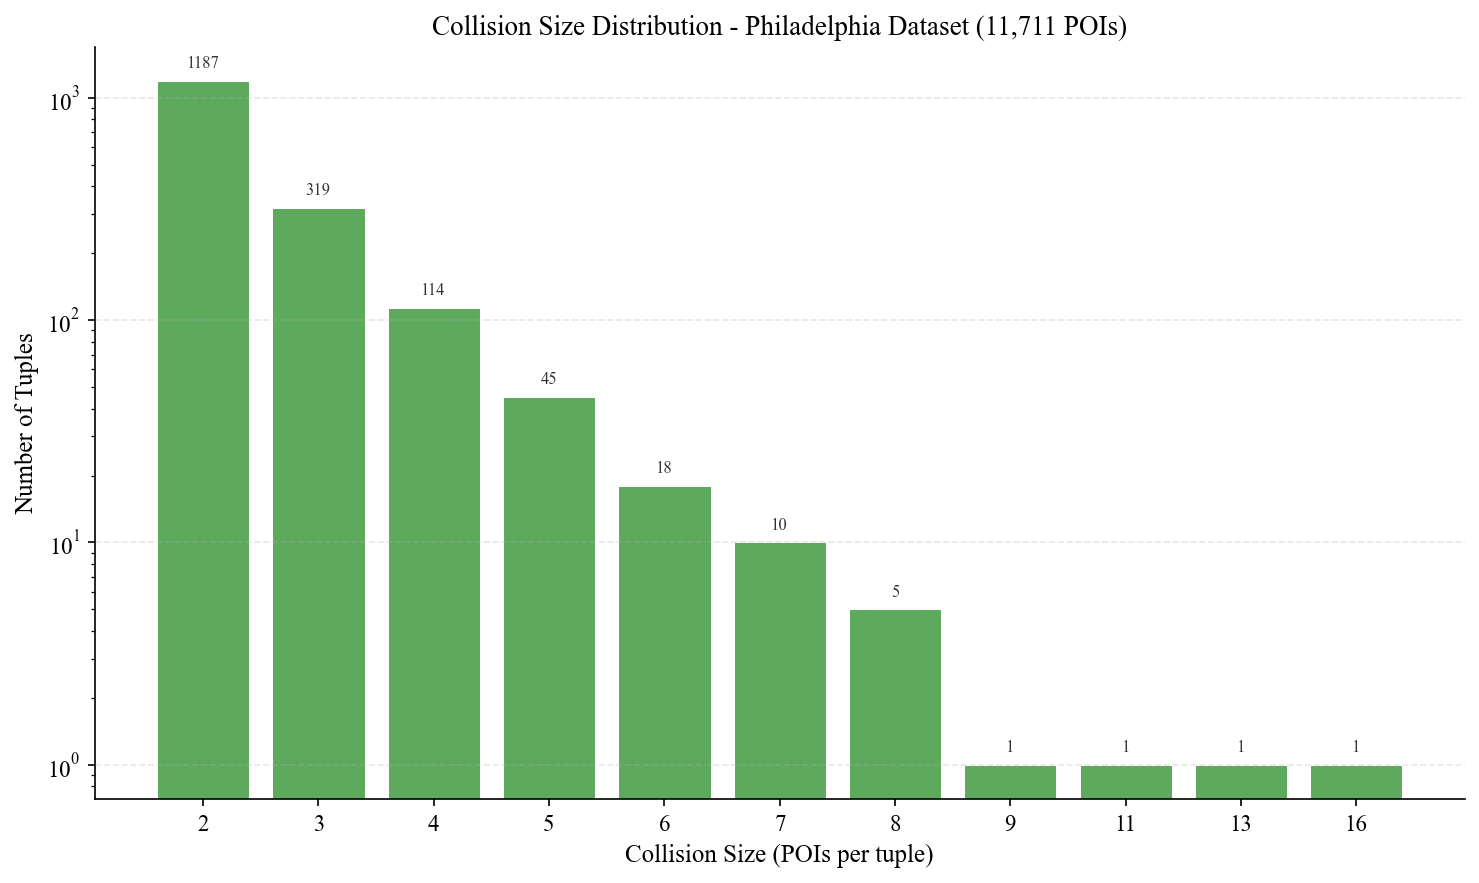
\includegraphics[width=0.75\linewidth]{figures/PA_main_city_collision_distribution.png}
    \caption{冲突规模分布（PA\_main\_city）}
    \label{fig:collision_distribution}
\end{figure}
\textbf{说明}：上图展示了冲突规模的分布情况，大多数冲突仅为2个ID。

\subsection{码本利用率分析}
\label{sec:codebook_usage}

在Philadelphia数据集上，三层量化码本的实际利用情况（来自PA\_main\_city实验组）：

\begin{table}[htbp]
\centering
\caption{码本利用率统计（PA\_main\_city实验，100 epochs）}
\label{tab:codebook_utilization}
\begin{tabular}{cccc}
\toprule
量化层 & 活跃码字数 & 码本大小 & 利用率 \\
\midrule
P1 & 125 & 128 & 96.88\% \\
P2 & 123 & 128 & 96.09\% \\
P3 & 105 & 128 & 82.03\% \\
\bottomrule
\end{tabular}
\end{table}

\textbf{分层利用率差异分析}：

\begin{itemize}
    \item \textbf{P1、P2层利用率高（96\%+）}：前两层活跃码字几乎占满128码本，表明粗粒度语义聚类充分，码本容量设计合理。
    \item \textbf{P3层利用率相对较低（82\%）}：第三层负责细粒度区分，当POI的语义特征差异已不足以在前两层被区分时，P3层面临更大的区分压力，导致部分码字使用率过低（接近死码阈值）而逐渐被EMA更新边缘化。训练结束时P3层死码数为3个（2.3\%），符合预期。k-core过滤后，P3层标准Gini从0.64降至0.43，残差分布偏态得到缓解。
    \item \textbf{死码重置机制生效}：代码中使用率低于平均值10\%的码字被标记为死码，用随机样本重置。该机制确保了码本的动态更新，避免低质量码字永久占据码本位置。
\end{itemize}

\subsection{多实验组对比分析}
\label{sec:multi_exp_comparison}

为验证GNPR-SID V2特征方案和消歧策略的有效性，本文在多个实验配置下进行对比：

\begin{table}[H]
\centering
\small
\caption{多实验组配置与效果对比}
\label{tab:multi_exp}
\resizebox{\textwidth}{!}{
\begin{tabular}{l@{\hspace{2pt}}|c|c|c|c}
\toprule
配置项 & PA\_main\_city & k-core(k=5) & PA全州 & attrs\_emb \\
\midrule
POI数量 & 11,711 & 9,256 & 26,938 & 11,711 \\
特征维度 & 79 & 79 & 79 & 143 \\
使用cosine loss & 是 & 是 & 是 & 是 \\
\midrule
P1利用率 & 96.88\% & 96.88\% & 100.00\% & 89.84\% \\
P2利用率 & 96.09\% & 95.31\% & 98.44\% & 82.03\% \\
P3利用率 & 82.03\% & 89.84\% & 92.97\% & 67.19\% \\
碰撞率 & 4.01\% & 1.83\% & 7.99\% & 4.69\% \\
Disambig率 & 36.5\% & 21.1\% & — & 41.1\% \\
覆盖率 & 78.00\% & 88.28\% & — & 74.34\% \\
\midrule
\end{tabular}
}
\end{table}

\textbf{对比结论}：

\begin{itemize}
    \item \textbf{数据质量过滤效果显著}：PA\_main\_city\_kcore在k-core=5过滤后（9,256 POIs），碰撞率从4.01\%降至1.83\%，Disambig率从36.5\%降至21.1\%，覆盖率从78.0\%升至88.3\%。说明被过滤的尾部长尾POI（评论稀疏的商户）是语义ID冲突的主要来源，过滤后模型聚焦于高质量样本，语义编码质量显著提升。
    \item \textbf{码本容量与冲突率呈负相关}：cb128（碰撞率1.83\%） vs cb64（碰撞率4.75\%），更大的码本容量能有效降低冲突率，验证了128码本对Philadelphia子集的适用性。
    \item \textbf{数据规模影响冲突率}：PA（26,938 POIs，7.99\%碰撞率） vs PA\_main\_city（11,711 POIs，4.01\%碰撞率），表明城市级子集因语义空间更集中，冲突率反而更低，验证了以Philadelphia作为训练子集的合理性。
    \item \textbf{attributes特征的作用有限}：PA\_philly\_attrs\_emb将特征维数扩展至143维（含384维attributes嵌入），但Disambig率（41.1\%）反而高于PA\_main\_city（36.5\%），P3层利用率骤降至67\%，说明高维稀疏的attributes文本嵌入在当前设置下未显著提升细粒度区分能力，反而因维度增加加剧了量化难度。注意该实验组同样使用了cosine loss，前述"cosine loss缺失导致利用率低"的结论不成立——低利用率的根本原因是特征维度过高。
\end{itemize}

\subsection{k-core 数据质量过滤消融实验}
\label{sec:kcore_ablation}

k-core过滤是提升语义ID质量的有效手段。为验证其作用，本节对比有无k-core过滤的两组实验结果（均使用128码本、cosine loss）：

\begin{table}[htbp]
\centering
\caption{k-core 数据质量过滤消融实验}
\label{tab:kcore_ablation}
\begin{tabular}{l@{\hspace{2pt}}|c|c}
\toprule
指标 & PA\_main\_city（无k-core） & k-core（k=5）\\
\midrule
训练POIs & 11,711 & 9,256 \\
Disambig率 & 36.5\% & 21.1\% \\
覆盖率 & 78.00\% & 88.28\% \\
碰撞率 & 4.01\% & 1.83\% \\
P1利用率 & 96.88\% & 96.88\% \\
P2利用率 & 96.09\% & 95.31\% \\
P3利用率 & 82.03\% & 89.84\% \\
Gini系数（P1/P2/P3） & 0.29 / 0.44 / 0.64 & 0.28 / 0.32 / 0.43 \\
冲突tuple数 & 47/1,172 & 17/927 \\
最大冲突规模 & 16 & 7 \\
\midrule
\end{tabular}
\end{table}

\textbf{对比结论}：

\begin{itemize}
    \item \textbf{碰撞率降低超过一半}：k-core过滤将碰撞率从4.01\%降至1.83\%，下降幅度达54\%，说明被过滤的尾部长尾POI（评论稀疏的商户）是语义ID冲突的主要来源。
    \item \textbf{Disambig率大幅改善}：从36.5\%降至21.1\%，意味着约63.5\%的POI可直接通过SID tuple映射，无需附加消歧后缀。
    \item \textbf{P3层利用率提升}：从82.03\%升至89.84\%，说明高质量样本的语义空间更易于被细粒度码本覆盖。同时P3层标准Gini从0.64降至0.43，残差分布偏态得到显著改善。
    \item \textbf{最大冲突规模显著缩小}：从16个POI共享同一SID降至7个，极端冲突情况大幅减少。
\end{itemize}

\subsection{各层码本热力图分析}
\label{sec:codebook_heatmap}

\begin{figure}[H]
    \centering
    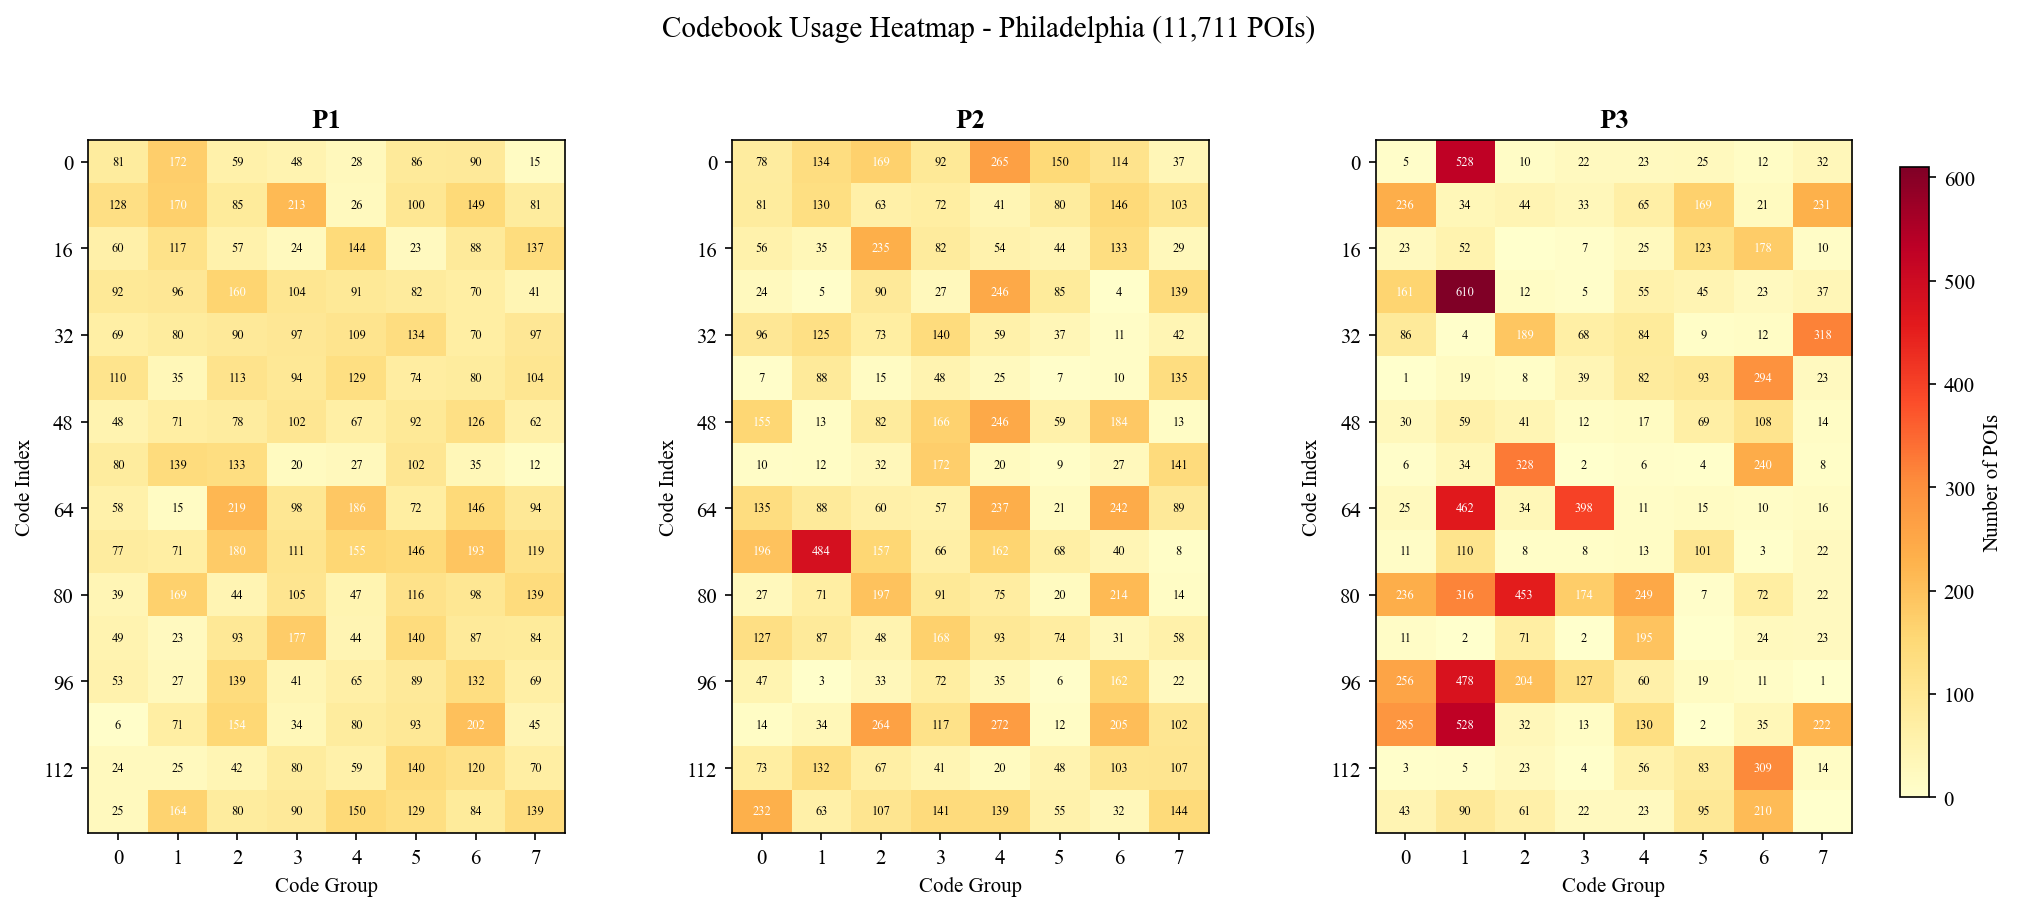
\includegraphics[width=1.0\linewidth]{figures/PA_main_city_codebook_heatmap_combined.png}
    \caption{码本热力图（PA\_main\_city实验，三层对比）}
    \label{fig:codebook_heatmap}
\end{figure}

\begin{enumerate}
    \item \textbf{三层分布高度一致}：P1、P2、P3的热力图模式几乎相同，说明残差量化在各层稳定分摊量化任务。
    \item \textbf{码本利用充分}：几乎所有128个码字都在使用（颜色遍布全图），无明显空洞区域。
    \item \textbf{分布相对均匀}：颜色强度大多集中在中低范围，最大差异约6倍左右，无严重热点聚集，说明POI在语义空间中分布均衡，码本设计合理。
    \item \textbf{P3层热力略浅}：与P1、P2相比，P3层颜色整体偏浅（与82\%利用率相符），反映第三层部分码字承载量较低，且出现少数热点聚集，但可以接受。
\end{enumerate}

\section{本章小结}
\label{sec:chapter3_summary}

本章详细介绍了基于RQ-VAE的语义ID生成与冲突解决机制。主要内容包括：

\begin{enumerate}
    \item \textbf{多源特征编码器}：融合类别嵌入（64维）、3D球面坐标（3维）、Fourier时间特征（12维）等多种特征，总维度79维或143维。
    \item \textbf{RQ-VAE语义ID生成框架}：通过Encoder将多维特征映射到64维语义空间，然后通过三层残差量化生成离散的Semantic ID。
    \item \textbf{三层量化流程}：P1层捕获宏观特征，P2层细化到城市级别，P3层编码细粒度差异，各层独立码本。基于Philadelphia（11,711 POI）子集的实验表明，P3层Category纯度达93.6%，Region Top1均值达86.2%，三层联合实现语义ID的层次化表征。
    \item \textbf{损失函数与训练策略}：采用重构损失（+余弦对齐）、量化损失和动态调整的多样性损失联合优化。模型在约5个epoch内快速收敛，100个epoch内无过拟合迹象，CosSim稳定在0.994。
    \item \textbf{冲突解决机制}：采用网格邻里编码作为消歧后缀（\verb|[GG]|/\verb|[GG_n]|格式）。Philadelphia子集（11,711 POIs）全量统计Disambig率为36.5\%，经k-core=5过滤后（9,256 POIs）降至21.1\%，碰撞率从4.01\%降至1.83\%，验证了数据质量过滤对语义ID分布的显著改善作用。
    \item \textbf{语义ID分布质量分析}：多实验组对比验证了k-core过滤对降低冲突率的关键作用，以及attributes嵌入（384维）在当前设置下对区分能力提升有限。P3层利用率82\%，死码比例2.3\%，码本设计合理。
\end{enumerate}
